\section{Client}
Ein Client ist ein Programm oder Gerät, dass auf einer Seite eines Netwerkes mit einem Browser auf der anderen kommuniziert.\\
 In diesem Fall ist dies ein Browser eines Besuchers der Seite. Das Gerät des Benutzers kann sowohl ein normaler PC als auch ein Smartphone oder ein Tablet sein. Die Schwiergkeit hier ist, dass eine Webseite auf beiden gut aussehen sollte. Da die Bildschirmgröße eines Smartphones deutlich geringer ist, muss der Inhalt entsprechend größer dargestellt werden. Notwendig is auch, dass Menüs, Schaltflächen, Links und mehr gut durch ein Touchinterface zu bedienen sind. Aus Gründen der Sicherheit und Privatsphäre kann ein Server aber nicht vor der eigentlichen Kommunikation zwischen diesen Gerätetypen unterscheiden. Während es theoretisch möglich ist, nach dem Herstellen einer Verbindung über \texttt{AJaX} Daten nachzuladen, ist es praktischer wenn die Seite eigenständig bestimmen kann, um welchen Gerätetyp es sich handelt. Dementsprechend ist eine Reaktion und Anpassung des Seitenlayouts nach dem Übertragen der Daten durch das Ausführen von Code durch den Client notwendig.\\

Ein weiteres Problem ist, dass die Seite ohne Serverunterstützung sämtliche Aufgaben durchführen können muss, für die eine erneute Datenübertragung schlichtweg zu zeitaufwändig wäre. Beispiele hierfür sind das Filtern nach bestimmten Lehrern beziehungsweise Klassen, das Anzeigen von Menüs und das Wechseln zwischen verschiedenen Tagen\\

Um eine Seite bei der Benutzung dynamisch und unabhängig zu machen, werden Stil- und Skriptsprachen verwendet. Die gebräuchlichen sind \texttt{CSS} und \texttt{JavaScript}.

\subsection{Abrufen der Daten vom Server}
Ruft ein Benutzer die Vertretungsplanseite mit dem richtigen Passwort auf, reagiert der Server, parst die Templatedatei und übermittelt dem Client mithilfe von \texttt{HTTPS} das HTML-Gerüst der Seite. Darin sind Verweise auf Stildateien und Skripte enthalten, die der Client darauffolgend beim Server erfragt. Zuletzt werden Bilder übertragen, da diese viel Speicherplatz beanspruchen und somit bei langsamen Internetverbindungen auch mehr Zeit zum Übermitteln benötigen, während die Seite auch ohne sie darstellbar ist. Der Browser wendet nun relativ komplexe Algorithmen an, um die Seite anzuzeigen und permanent zu aktualisieren. Im Hintergrund beginnt ein \JavaScript-Interpreter die angeforderten Skripte auszuführen.
\subsection{Design}
Das Design ist eine der Aufgaben, die die größte Menge an Code erfordern. Jedem \HTML-Tag muss mithilfe von \CSS vermittelt werden, wie er auf dem Bildschirm dargestellt werden soll. Das ganze reicht von Farben, Rahmen und Abständen bis hin zu komplexen Animationen und Transformationen. Die Syntax von \CSS ist dabei sehr einfach:\\\\
\texttt{selektor \{\\anweisung: wert;\\anweisung: wert;\\\}}\\\\
Mit dem Selektor wird ausgewählt, welche Tags angesprochen werden. Das können beispielsweise alle Kindelemente eines Link-Tags (\texttt{a>*}), das Element mit der ID section (\texttt{\#section}) oder alle Elemente und Unterelemente der table-Klasse sein (\texttt{.table, .table *}). Mit sogenannten Pseudoklassen lassen sich auch beispielsweise nur Elemente auswählen, die sich unter dem Mauszeiger befinden oder angeklickt werden.\\
Die folgenden Schlüssel-Wert-Paare geben die für die ausgewählten Elemente anzuwendenden Stilregeln an.\\
\begin{center}
	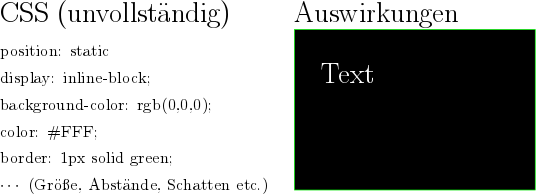
\includegraphics[width=0.75\textwidth]{texte/res/1.png}
\end{center}
Durch das Verwenden vieler solcher Blöcke lässt sich jede Webseite darstellen.\\
\subsubsection{Anwendung}
Die Seite ist in einen Seitentitel mit Menü und den Hauptteil der Seite, den eigentlichen Vertretungsplan unterteilt. Dieser besteht aus einer dynamisch generierten \CSS-Tabelle.
\subsubsection{Tabelle}
%


\subsection{Interaktivität}
%%
\subsubsection{Filter}
%
\subsubsection{Cookies}
%
\subsubsection{Menü}
%

%EOF
